\section{Experiment 8D: privacy-utility recovery}
\label{sec:experiment8d}

\paragraph{Question and fixed privacy statement.}
Experiment 8D tests whether the failed 8C utility gate can be recovered without
weakening its privacy definition. The protected unit remains one vehicle's
complete local dataset, adjacency remains replacement of one client, and
$\delta=10^{-5}$. The same analytic Gaussian calibration and one-shot family
mean release are used. Consequently, the only sensitivity reductions are a
smaller public log-parameter box and larger compatible secure-aggregation
cohorts; neither is a change from client-level to record-level privacy.

\paragraph{Protocol.}
The broad box from 8C is compared with the public benchmark-design box
$C_f/m\in[40,70]$, $C_r/m\in[35,75]$, and $m/I_z\in[0.45,0.8]$.
The latter is fixed from the declared admissible fleet design and is not fitted
to a participating client's records. Clipping remains part of the mechanism,
so the privacy guarantee also holds for an out-of-box contribution. No local
coordinate was clipped in this run. Tight-box cohorts contain 10, 30, or 100
clients per oracle family, with complementary speeds balanced over 10--30 m/s.
Five independent training fleets (seeds 81--85) are evaluated on separately
generated ten-client-per-family test fleets. Each finite
$\epsilon\in\{2,4,8\}$ uses ten privacy draws. The unchanged gate requires at
most 10\% mean tracking degradation relative to that mechanism's non-private
mean, full amplitude feasibility, and worst frozen spectral radius below one.

\begin{table}[htbp]
\centering
\caption{Experiment 8D privacy recovery. Tracking is mean yaw-rate RMSE in
deg/s. Increase is relative to the matching non-private cohort mean.}
\label{tab:experiment8d}
\begin{tabular}{llrrrr}
\toprule
Bounds/cohort & $\epsilon$ & Tracking & Increase & Feasible & Max. $\rho$\\
\midrule
Broad/10 & 2 & 0.37199 & 4632.12\% & 1.00 & 1.0457\\
Broad/10 & 4 & 0.14915 & 1797.37\% & 1.00 & 0.9913\\
Broad/10 & 8 & 0.06578 & 736.80\% & 1.00 & 0.9764\\
Tight/10 & 2 & 0.02162 & 174.99\% & 1.00 & 0.9732\\
Tight/10 & 4 & 0.01564 & 98.95\% & 1.00 & 0.9714\\
Tight/10 & 8 & 0.01100 & 39.91\% & 1.00 & 0.9703\\
Tight/30 & 2 & 0.01088 & 39.82\% & 1.00 & 0.9707\\
Tight/30 & 4 & 0.00908 & 16.60\% & 1.00 & 0.9698\\
Tight/30 & 8 & 0.00827 & 6.22\% & 1.00 & 0.9695\\
Tight/100 & 2 & 0.00825 & 6.05\% & 1.00 & 0.9692\\
Tight/100 & 4 & 0.00783 & 0.62\% & 1.00 & 0.9690\\
Tight/100 & 8 & 0.00779 & 0.09\% & 1.00 & 0.9688\\
\bottomrule
\end{tabular}
\end{table}

\begin{figure}[htbp]
\centering
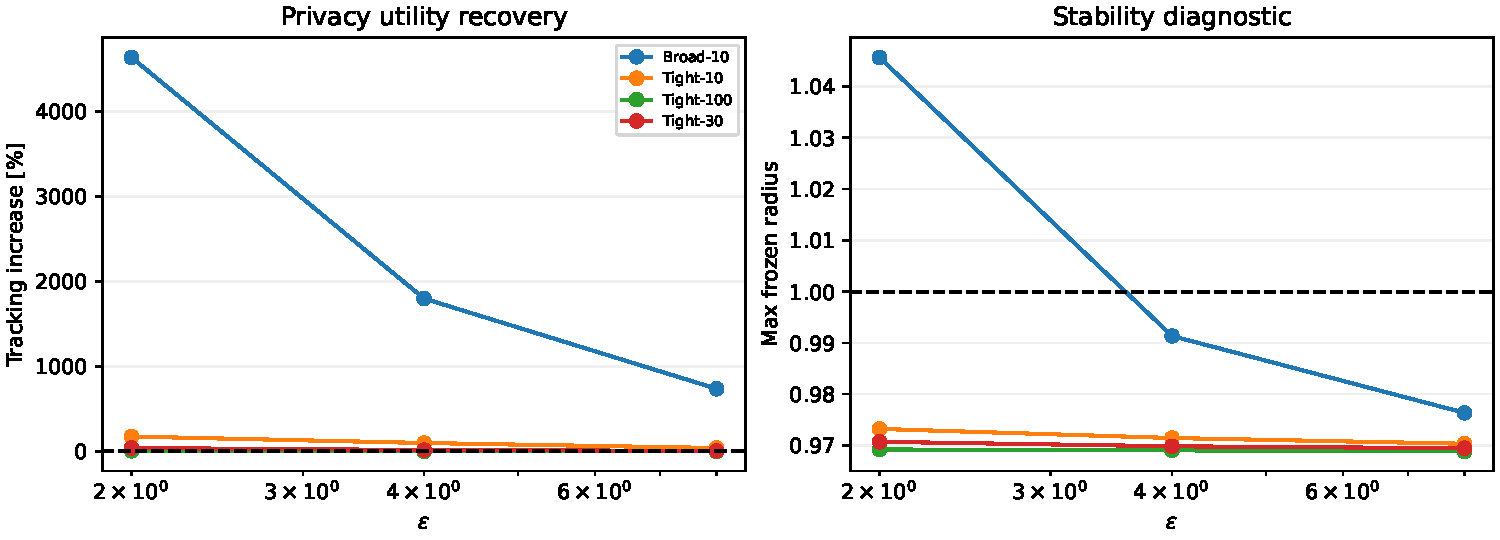
\includegraphics[width=0.9\linewidth]{../results/figures/experiment_8d_privacy_recovery.pdf}
\caption{Recovery from public bounds and cohort scaling. The left dashed line
marks the fixed 10\% tracking gate; the right dashed line marks frozen radius
one.}
\label{fig:experiment8d}
\end{figure}

\paragraph{Results.}
All 1,500 local fits converge. The run contains 1,860 family releases and
55,800 client--scenario evaluations. Tight/100 passes at every tested privacy
budget: degradation is 6.05\% at $\epsilon=2$, 0.62\% at $\epsilon=4$, and
0.09\% at $\epsilon=8$. Tight/30 first passes at $\epsilon=8$ with 6.22\%
degradation. Tight bounds alone greatly improve the ten-client result, but its
best finite cell still degrades tracking by 39.91\%. All cells are
amplitude-feasible, although Broad/10 at $\epsilon=2$ fails the frozen-radius
criterion. Thus the recovery gate passes because sensitivity scales as $1/n$
and the defensible box reduces the physical magnitude represented by a fixed
normalized perturbation.

\paragraph{Interpretation and limitations.}
The result supplies a concrete FL privacy benefit: compatible vehicles can
share a useful client-level-DP family model while retaining their trajectories
locally, provided the aggregation cohort is sufficiently large. It is not
evidence that ten-client fleets are adequate, that family labels can be exposed
safely, or that production secure aggregation has been implemented. Cohort
sizes 30 and 100 are simulated availability assumptions with full participation;
dropout, malicious clients, privacy accounting across repeated releases, and
learned private clustering remain open. The relative gate is also stringent
because non-private tracking is about 0.0078 deg/s; application-specific safety
limits should be established independently rather than inferred from this sweep.

\paragraph{Decision and reproducibility.}
Experiment 8D passes its recovery gate. The strongest tested passing point is
$\epsilon=2$ with 100 clients per family. This justifies proceeding to a
federated system study that treats cohort formation, partial participation, and
repeated releases explicitly. The frozen protocol is
\path{code/config/experiment_8d.json}; the runner is
\path{code/experiments/experiment_8d_privacy_recovery.py}; and aggregate results
are retained in \path{results/tables/experiment_8d_summary.csv} with compressed
per-seed fits, releases, and client metrics available from a full run.
